\chapter{Simulating High Fidelity Rubin Donut Images}
\label{chap:sim}
\chaptermark{Simulating Donut Images}

% \epigraph{The first principle is that you must not fool yourself and you are the easiest person to fool.}{Richard Feynman}

\epigraph{Perhaps one day we will have machines that can cope with approximate task descriptions, but in the meantime, we have to be very prissy about how we tell computers to do things.}{Richard Feynman}

Simulation is a cornerstone of this work. The Rubin Observatory is not complete, which in some sense necessitates using simulated data. However, even if the observatory was complete and we could collect real data, it would still be challenging to adequately sample the 50 dimensional state space of the telescope. In real life, to configure the Rubin telescope in a perturbed state takes on the order of 10 seconds. In code, initializing a telescope instance in a specific configuration takes single digit microseconds. In real life, there is only one telescope, whereas using the Sherlock cluster at Stanford University, we can initialize the telescope in up to roughly one thousand parallel processes. In short, we exploit simulation to create richer datasets to train and assess our framework.

In the first section, we describe the details of simulating a single donut. In the following sections, we describe the two datasets used in this work. 

\section{Simulating A Single Donut Image}

We use high fidelity Rubin Observatory image simulations to train our model and analyze its performance. By selecting different observational, atmospheric, and telescope parameters for each donut, we produced a simulated training dataset that spans a wide variety of conditions. The output of each simulation $i$ is a $256 \times 256$ pixel donut image $D_i$, and the corresponding true local wavefront $\alpha_i \in \mathbb{R}^{18}$. Figure \ref{fig:donut} shows an example pair of end products. 
% 
\begin{figure} [!htbp]
\begin{center}
\begin{tabular}{c}
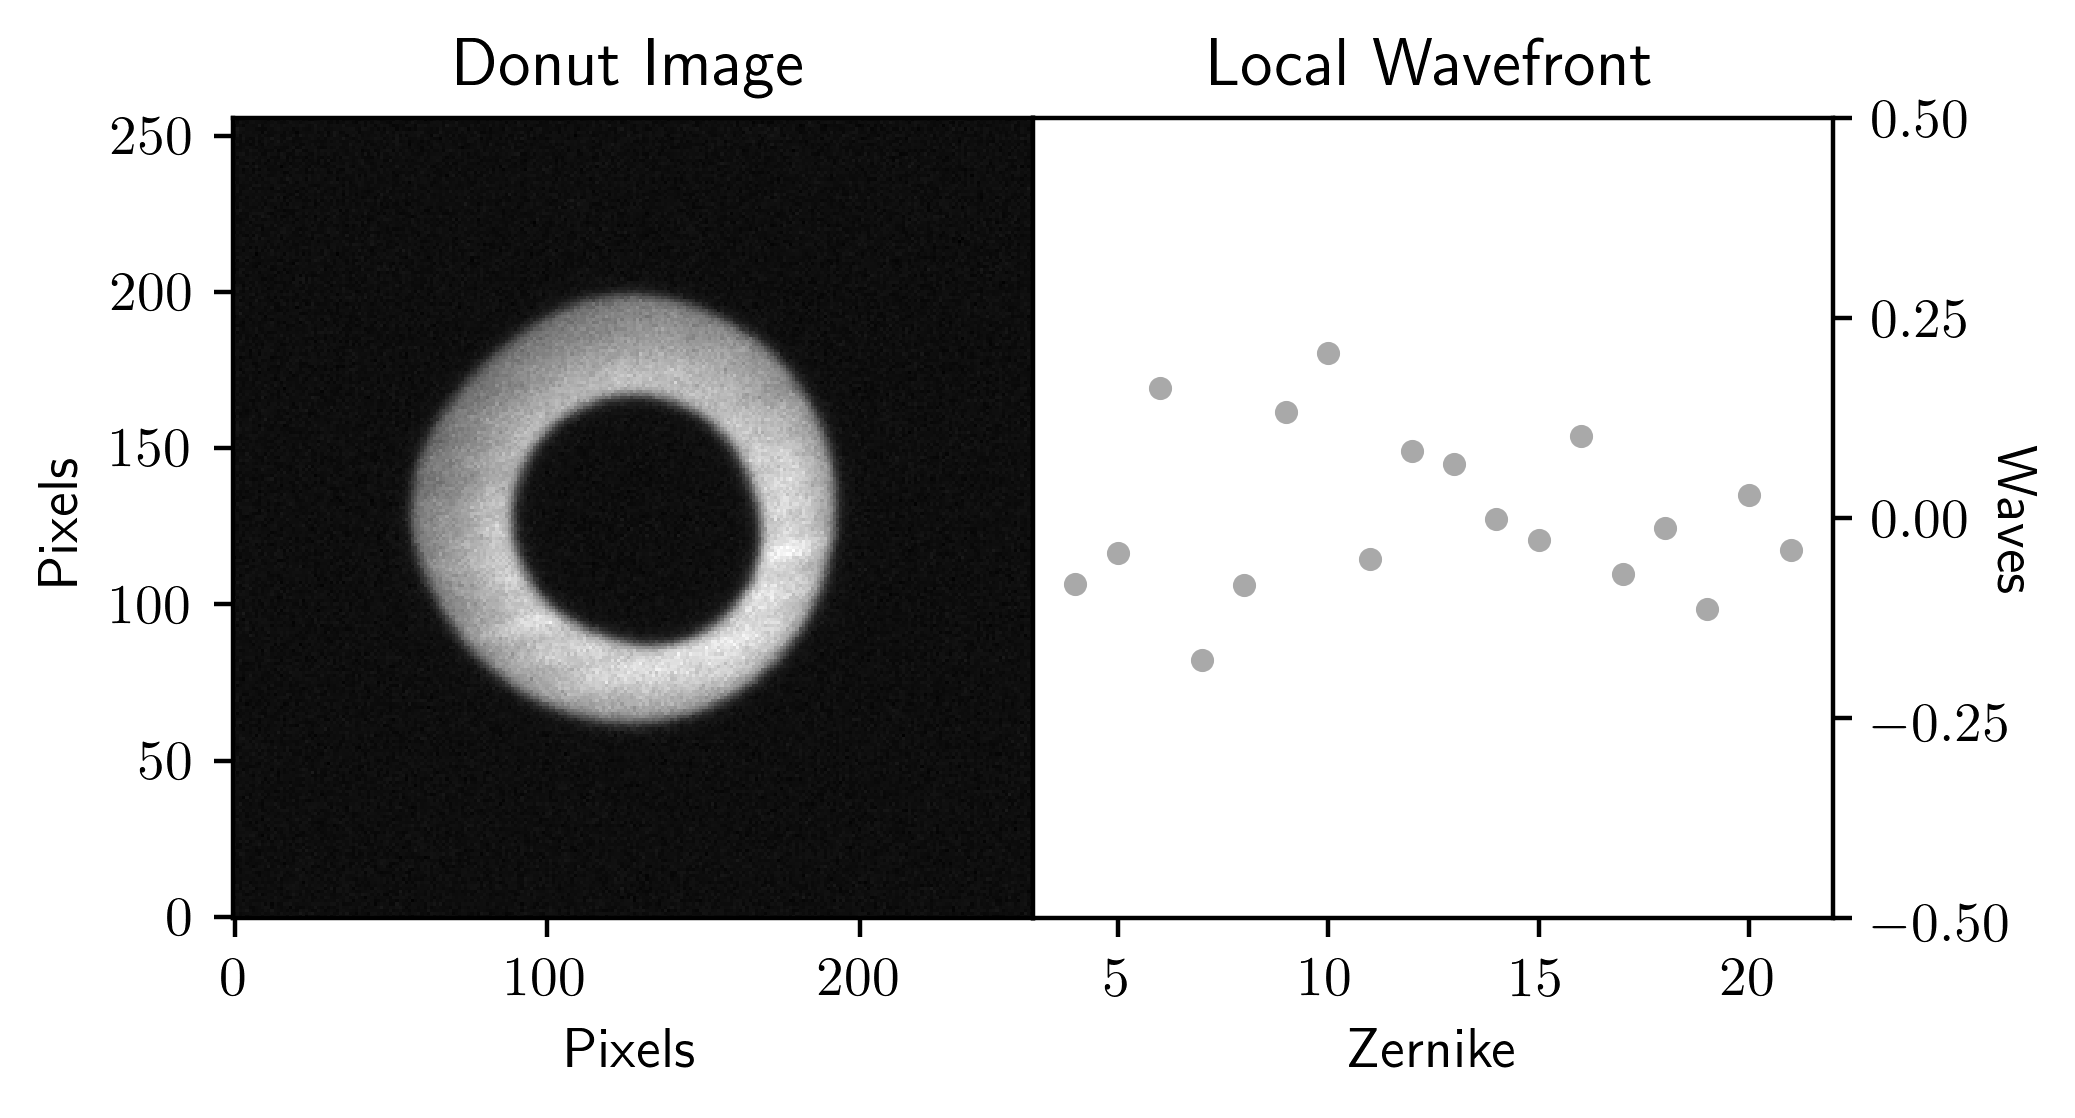
\includegraphics[width=6in]{figs/simulating_donuts/example_atm.png}
\end{tabular}
\end{center}
\caption[Simuated Donut and Local Wavefront]{\textit{Left:} a simulated $256\ \times\ 256$ pixel donut image at the $(x,y)$ field position ($-1.1048^o$, $1.0868^o$). \textit{Right:} the corresponding local wavefront annular Zernike coefficients ($Z_4-Z_{21}$ inclusive), measured in units of 622.20 nm waves. \label{fig:donut}}
\end{figure}

\begin{figure} [!htbp]
\begin{center}
\begin{tabular}{c}
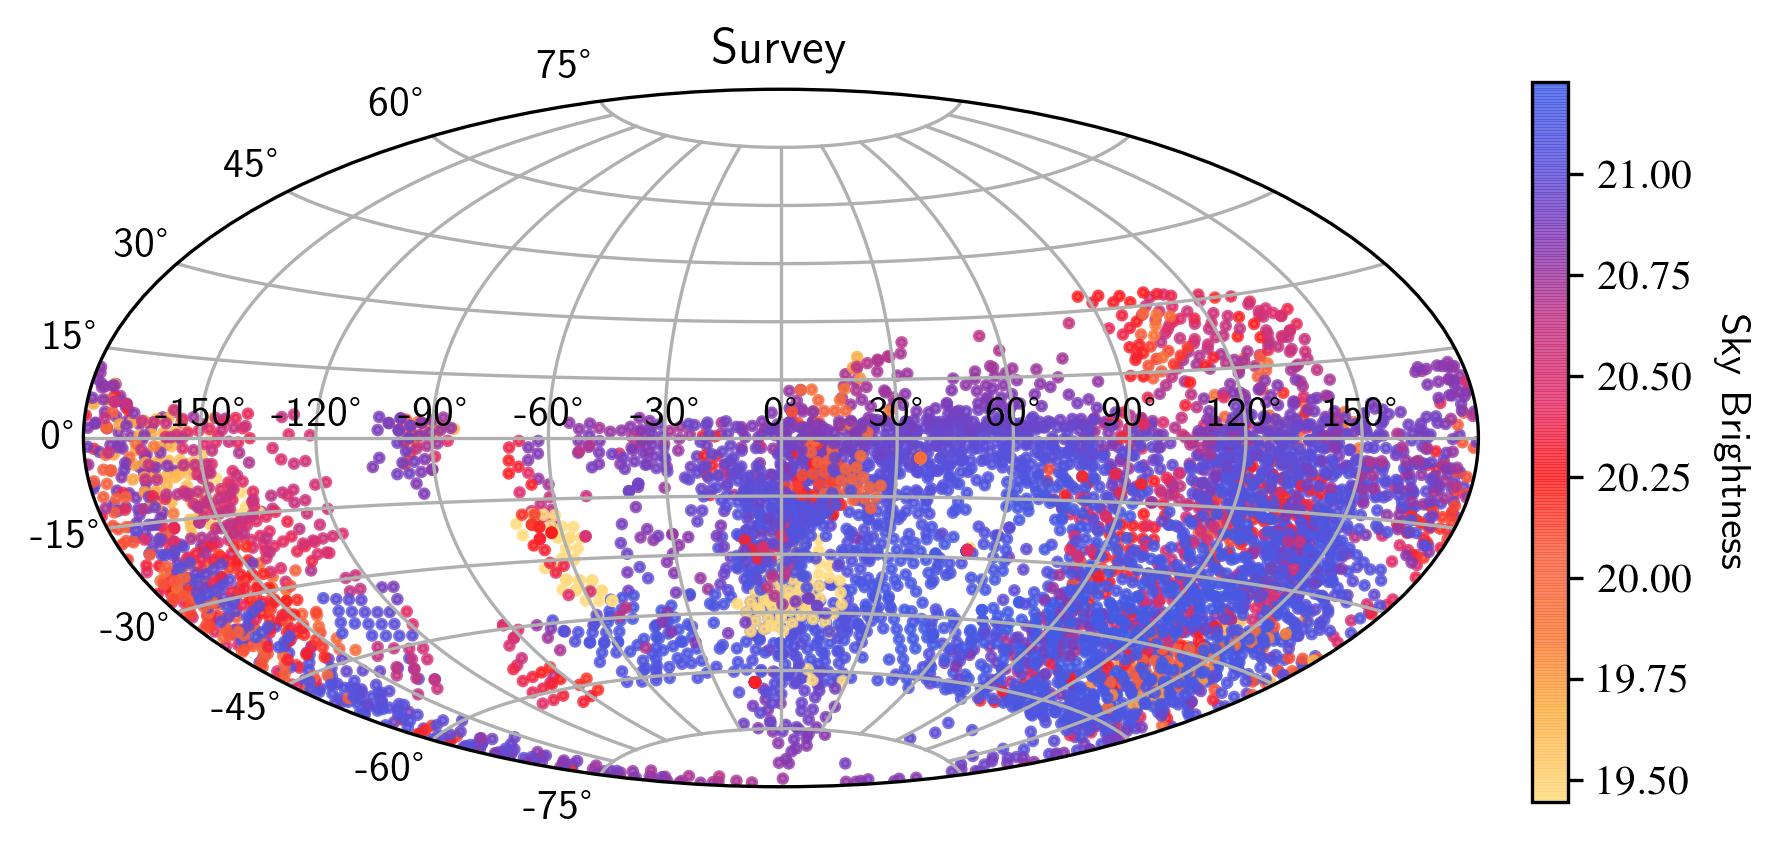
\includegraphics[width=6in]{figs/simulating_donuts/survey.png}
\end{tabular}
\end{center}
\caption[Survey Footprint]{The right ascension and declination of the observations we use for our simulations. Each point corresponds to an observation; the color shows the variation in sky brightness.\label{fig:survey}}
\end{figure}

The simulations are comprised of sequential steps that trace a photon's journey from a distant source to a count in a pixel in an image. The first step is to generate photons in the sky corresponding to a source from the observation. We create a baseline survey to draw observations from. The survey is comprised of 5497 randomly drawn r-band visits from the Operations Simulator (OpSim) \cite{opsim}. Figure \ref{fig:survey} shows the distribution of the observations across the sky. This survey samples a wide range of sky brightnesses, atmospheric seeing, and sky positions. 

For each of these visits, we determine the fields of view covered by the four corner wavefront sensors. Then we query the Gaia DR2 catalog for sources within these regions and with G magnitudes less than 18 \cite{dr2}. The mean number of sources per catalog is $1101$ with a standard deviation of $1720$. The largest catalog contains $12684$ sources. Once we have the catalog, we convert the Gaia $G$, $G_{bp}$, and $G_{rp}$ magnitudes to the SDSS $r$ magnitude based on Equation \ref{eqn:conversion} from the Gaia data release documentation \cite{conversion}.

\begin{align}\label{eqn:conversion}
x &= G_{bp} - G_{rp}\\
r &= G + 0.12879 - 0.24662 \cdot x + 0.027464 \cdot x^2 + 0.049465 \cdot x^3
\end{align}

\noindent We clip SDSS $r$ magnitudes below 14 to save simulation time. The simulation starts by selecting a source and generating the corresponding photons. The number of photons is determined by the SDSS magnitude and the wavelengths are drawn from a black body distribution with spectral radiance,

\begin{equation}\label{eqn:blackbody}
B(\lambda, T) = \frac{2hc^2}{\lambda^5}\frac{1}{e^{\frac{hc}{\lambda k_B T}} - 1}
\end{equation}

\noindent based on the temperature of the source. After the photons are generated, the next stage of simulation propagates them through the atmosphere.

The primary contribution from the atmosphere is atmospheric turbulence. We use the GalSim Python package to split the atmospheric turbulence power spectrum into low and high spatial frequencies and simulate their contribution separately \cite{galsim}. The low spatial frequencies modulate the centroid of the source photons. The high spatial frequencies scatter the photons around this centroid, sometimes called the \textit{second kick} \cite{phosim}. The phase screens are initialized with altitudes and velocities from atmospheric tomography profiles \cite{atmosphere}. The Fried parameter for the atmosphere is determined by the airmass and seeing from the OpSim observation and by the central wavelength of the $r$ bandpass, $622.20\ nm$. 

In addition to the turbulence contribution, we also incorporate chromatic seeing and differential chromatic refraction \cite{chromatic}. Both of these are functions of the wavelengths of individual photons. We model chromatic seeing by scaling the turbulence induced perturbations based on wavelength. We model chromatic refraction by refracting the photons along the meridian based on the airmass. At the conclusion of this step, there is a bundle of photons at the entrance pupil of the telescope.

Next, we trace photons from the entrance pupil of the primary mirror to the plane of the detector. The batoid Python package was used to construct model Rubin telescope instances and perform the ray tracing \cite{batoid}. We constructed telescope instances that have 50 degrees of freedom that are analogous to those in Table \ref{tab:dof}. For simplicity, we used 20 Zernike polynomials ($Z_4 - Z_{23}$) to represent the surface bending modes. We skip the first three Zernike modes because these surface perturbations would be degenerate with the hardpoint control parameters.

In order to determine a reasonable range for the degrees of freedom, we first computed the single parameter excitation levels, shown in Table \ref{tab:range}, that induce the global wavefront to have root-mean-square error of 0.3 wavelengths, or \textit{waves}. We set the amplitude of a given parameter by drawing from a normal distribution that is centered on the center of the range and has a standard deviation of half the range multiplied by $\sqrt{5/50}$. This means that the total error across all the control parameters will be roughly 5 times the error that on an individual parameter would make the global wavefront 0.3 waves (where a wave is the central wavelength of the r bandpass, or 622.20 nm).

\begin{table}[!htbp]
\caption[Range of Simulated Control Parameters]{\label{tab:range}The range in each degree of freedom where the root-mean-square of the global wavefront is below 0.3 waves (one wave is 622.20 nm). These ranges are used to create realistically deformed telescope instances in our simulations. Notation: dx is a translation in the x-axis; rx is a rotation along the x-axis; $Z_4$ is the fourth annular Zernike polynomial over the annulus of the corresponding surface.} 
\begin{center}
% \small
\begin{tabular}{|l|c|c|l|c|c|r|}
\hline
Parameter & Min & Max & Parameter & Min & Max\\
\hline
Camera dx \hfill (um) & -580 & 580 & M2 dx \hfill (um) & -118 & 118 \\
Camera dy \hfill (um) & -580 & 580 & M2 dy \hfill (um) & -118 & 118 \\
Camera dz \hfill (um) & -10.7 & 5.39 & M2 dz \hfill (um) & -11.1 & 11.1 \\
Camera rx \hfill (urad) & -42.0 & 42.0 & M2 rx \hfill (urad)& -17.6 & 17.6 \\
Camera ry \hfill (urad) & -42.0 & 42.0 & M2 ry \hfill (urad) & -17.6 & 17.6 \\
M1M3 $Z_4 $\hfill (nm) & -111 & 56.4 & M2 $Z_4 $ \hfill (nm) & -59.1 & 117 \\
M1M3 $Z_5 $\hfill (nm) & -42.4 & 42.4 & M2 $Z_5 $ \hfill (nm) & -68.9 & 68.9 \\
M1M3 $Z_6 $\hfill (nm) & -42.4 & 42.4 & M2 $Z_6 $ \hfill (nm) & -68.9 & 68.9 \\
M1M3 $Z_7 $\hfill (nm) & -65.0 & 65.0 & M2 $Z_7 $ \hfill (nm) & -76.4 & 76.4 \\
M1M3 $Z_8 $\hfill (nm) & -65.0 & 65.0 & M2 $Z_8 $ \hfill (nm) & -76.4 & 76.4 \\
M1M3 $Z_9 $\hfill (nm) & -45.9 & 45.9 & M2 $Z_9 $ \hfill (nm) & -70.6 & 70.6 \\
M1M3 $Z_{10}$ \hfill (nm) & -45.9 & 45.9 & M2 $Z_{10} $ \hfill (nm) & -70.6 & 70.6 \\
M1M3 $Z_{11}$ \hfill (nm) & -130 & 66.2 & M2 $Z_{11} $ \hfill (nm) & -62.8 & 70.4 \\
M1M3 $Z_{12}$ \hfill (nm) & -51.5 & 51.5 & M2 $Z_{12}$ \hfill (nm) & -68.3 & 68.3 \\
M1M3 $Z_{13}$ \hfill (nm) & -51.5 & 51.5 & M2 $Z_{13}$ \hfill (nm) & -68.3 & 68.3 \\
M1M3 $Z_{14}$ \hfill (nm) & -48.1 & 48.1 & M2 $Z_{14}$ \hfill (nm) & -73.6 & 73.6 \\
M1M3 $Z_{15}$ \hfill (nm) & -48.1 & 48.1 & M2 $Z_{15}$ \hfill (nm) & -73.6 & 73.6 \\
M1M3 $Z_{16}$ \hfill (nm) & -73.6 & 73.6 & M2 $Z_{16}$ \hfill (nm) & -68.0 & 68.0 \\
M1M3 $Z_{17}$ \hfill (nm) & -73.6 & 73.6 & M2 $Z_{17}$ \hfill (nm) & -68.0 & 68.0 \\
M1M3 $Z_{18}$ \hfill (nm) & -49.7 & 49.7 & M2 $Z_{18}$ \hfill (nm) & -64.8 & 64.8 \\
M1M3 $Z_{19}$ \hfill (nm) & -49.7 & 49.7 & M2 $Z_{19}$ \hfill (nm) & -64.8 & 64.8 \\
M1M3 $Z_{20}$ \hfill (nm) & -49.2 & 49.2 & M2 $Z_{20}$ \hfill (nm) & -76.5 & 76.5 \\
M1M3 $Z_{21}$ \hfill (nm) & -49.2 & 49.2 & M2 $Z_{21}$ \hfill (nm) & -76.5 & 76.5 \\
M1M3 $Z_{22}$ \hfill (nm) & -67.7 & 51.5 & M2 $Z_{22}$ \hfill (nm) & -59.0 & 57.2 \\
M1M3 $Z_{23}$ \hfill (nm) & -51.3 & 51.3 & M2 $Z_{23}$ \hfill (nm) & -65.7 & 65.7 \\
\hline
\end{tabular}
\end{center}
\end{table} 

Once the photons are at the detector, we simulate sensor effects. We use GalSim to simulate the aggregation of photons into silicon pixels. The silicon model includes electron diffusion to account for the nonlinear brighter-fatter effect \cite{brighterfatter}. We also use GalSim to introduce shot noise from the sky background and simulate the camera readout. Then we zero both individual pixels and columns following sensor statistics taken in the lab. At this point, we have a $256 \times 256$ pixel digital image of counts like the one shown in Figure \ref{fig:donut}.

For each donut image, we also simulate the corresponding local wavefront. We use the Batoid package to compute the wavefront at the donut's field position $x,y$. The local wavefront $\alpha$ is represented by the 18 annular Zernike coefficients which have the largest impact on image quality ($Z_4 - Z_{21}$ inclusive). These coefficients serve as the labels for the neural network described in the next Chapter.

In addition to donuts from individual stars, we also simulated blended donuts. These arise when the donut images from two or more stars overlap. In these simulations, the photons from all the overlapping stars are aggregated on the sensor, then the sensor effects are simulated once. In crowded fields, the majority of the donuts will be blends. This data helps us assess this scenario and the density limits of the fields where we can successfully apply our algorithm. 

In the next two Sections we describe the datasets used to train the neural network and to test the full framework, respectively.

% We believe these simulations capture the core attributes of individual donut images and their corresponding wavefronts. There are two ways we can make these simulations more holistic in future work. The first is to include blending from overlapping donuts. In this work, we process each donut individually, whereas in real operation we expect many of the donuts to be blended. The second is using multiple bands. All the analysis in this work is done on images from the r-band. We believe that after demonstrating the efficacy of this technique in the r band, we will be able to easily extend the model to the other bands with transfer learning.

\section{Donut Dataset}

The donut dataset consists of samples with three components: the simulated donut image $D$, the focal plane position $r$ - which includes distance along the focal $z$ axis, and the true local wavefront $\alpha$. The dataset is used to train, validate, and test models for the task,

\begin{equation}\label{eqn:blackbody}
(D,r) \to \alpha
\end{equation}

Modern neural networks, like the one we develop in Chapter \ref{chap:cnn}, typically have millions of parameters. In order to constrain these parameters and simultaneously avoid overfitting, these models must be trained on copious amounts of data. 

For each of the first 5,000 visits from the observing schedule, we simulate 200 individual donut images. The most computationally expensive part of these simulations is generating the atmospheric phase screens. We speed up the simulations by using one atmosphere for every 100 donuts. Telescope instantiation, on the other hand, costs a few microseconds, so we draw a different 50-dimensional perturbation to the nominal telescope state for each donut image. We also simulate 100,147 blends from the same observations. 

Following the standard machine learning cross validation paradigm, we break this data up into training, validation, and test segments. The training, validation, and test sets are comprised of 498,071 stars and 100,028 blends, 220 stars and 36 blends, and 1,708 stars and 340 blends respectively. Figure \ref{fig:donutbox} shows 100 example donuts from the training set. 

\begin{figure} [!htbp]
\begin{center}
\begin{tabular}{c}
\includegraphics[width=\textwidth]{figs/simulating_donuts/huge_donut_box.png}
\end{tabular}
\end{center}
\caption[Example Donuts from Donut Dataset]{Example donuts from the training set. The different degrees of vignetting, missing columns, blending, and turbulence can be seen with the naked eye.\label{fig:donutbox}}
\end{figure}

\section{Full Visit Dataset}

The full problem involves going from $n$ donut images and positions to the 54 coefficients $\beta$,

\begin{equation}\label{eqn:blackbody}
(D_1,r_1), \dots, (D_n, r_n) \to \alpha_1, \dots, \alpha_n \to \beta
\end{equation}

\noindent In addition to the donut dataset, we also need a dataset of full visits, where each visit contains many donut images, so that we can assess how well our framework predicts $\beta$.

Each sample in this dataset consists of all the donut images and positions in the observation, plus the full optics wavefront $\beta$. We used the last 497 observations from the scheduler simulations for the observations. For each visit, we simulated all the stars, and blends, from the Gaia catalog that fall on the corner wavefront sensors. The mean, median, and maximum number of sources in a sample is 787, 222, and 4,998 respectively. Figure \ref{fig:sensordonut} shows an example sample.

\begin{figure} [!htbp]
\begin{center}
\begin{tabular}{c}
\includegraphics[width=\textwidth]{figs/simulating_donuts/sensors_and_donuts.png}
\end{tabular}
\end{center}
\caption[Example Full Visit Sample]{The eight wavefront sensor half-chips in an example sample from the full visit dataset. This sample contains 1112 donut images which are highlighted in blue boxes. \label{fig:sensordonut}}
\end{figure}

All the donuts within a single observation are simulated with the same atmosphere and sky background. Otherwise, each star in the observation is simulated in the same manner as the donuts dataset described above. For each observation, we used the batoid framework to compute the optics wavefront double Zernike coefficients for the perturbed telescope instance.

The largest difference between observations is the density of sources in the field. The number of sources in a sample ranges from 111 to 4998. On average, 32 percent of the sources are blends. However, for the crowded fields this number can be over 90 percent. Figure \ref{fig:blendfraction} shows how the fraction of sources that are blends increases with the total number of sources in the visit. Thus, while for less crowded fields ample un-blended stars are available, for crowded fields, the wavefront sensing algorithm's ability to process blends is critical.

\begin{figure} [!htbp]
\begin{center}
\begin{tabular}{c}
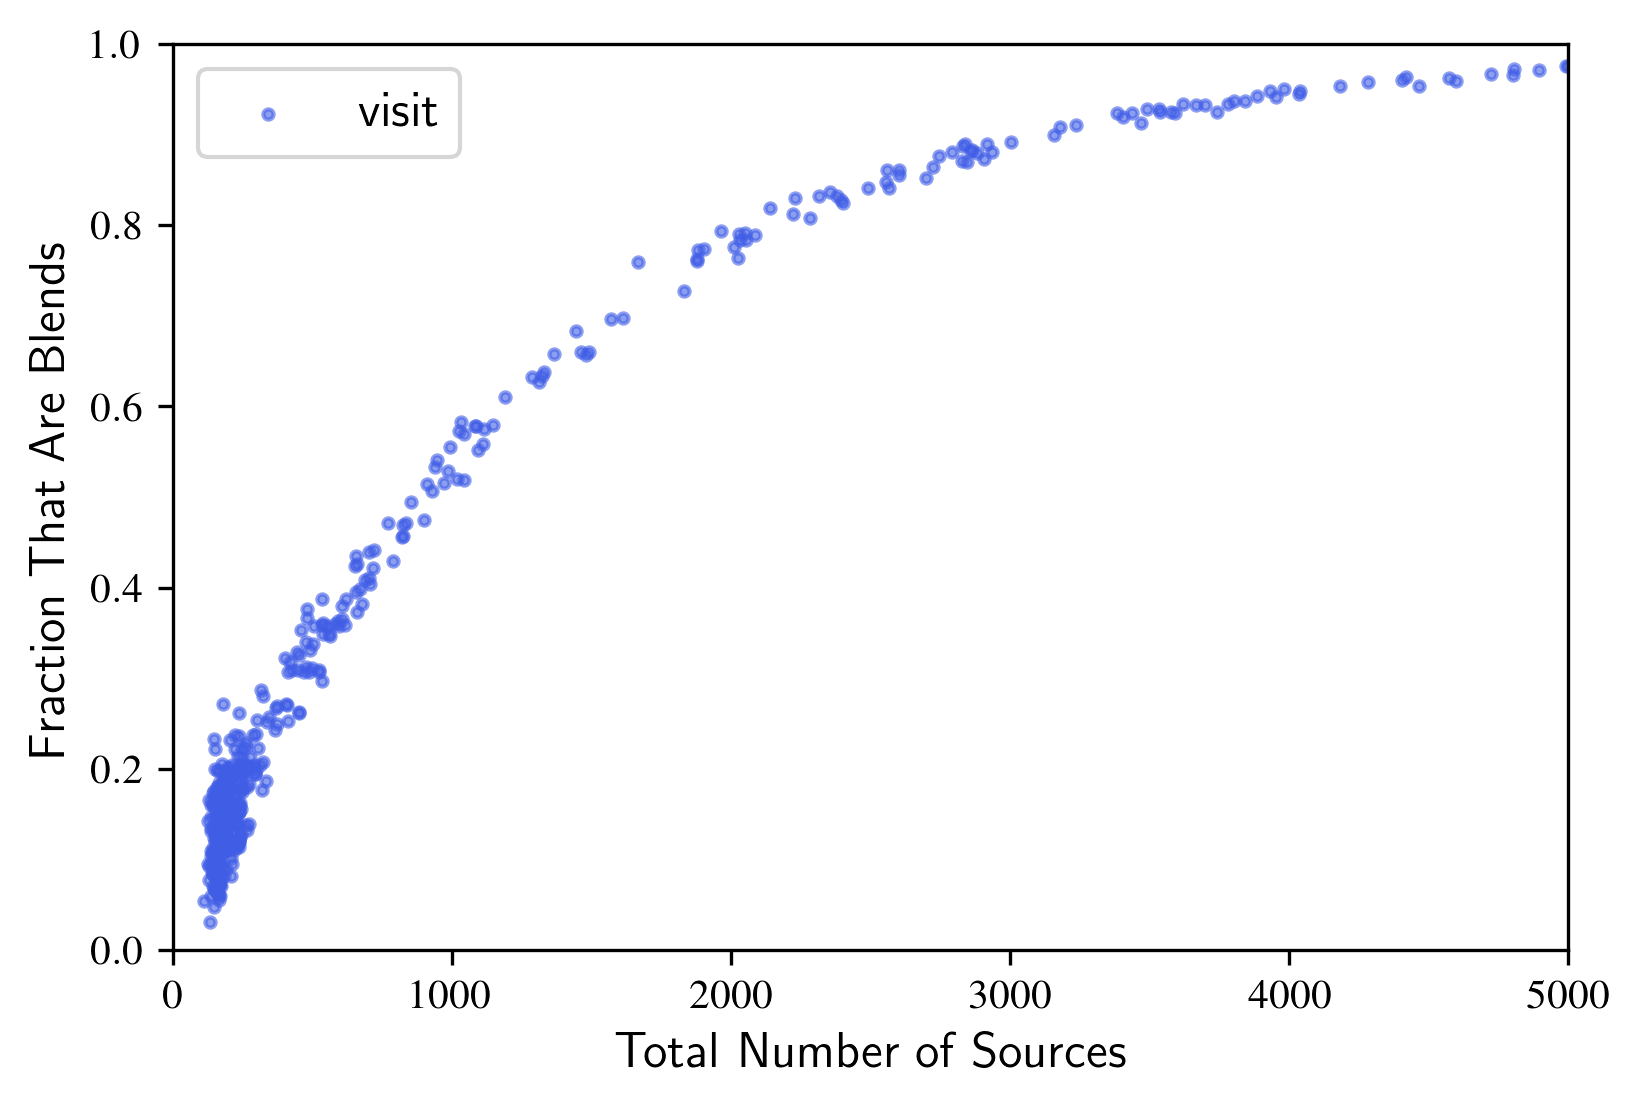
\includegraphics[width=\textwidth]{figs/simulating_donuts/blendfraction.png}
\end{tabular}
\end{center}
\caption[Fraction of Blended Sources]{The fraction of sources that are blends versus the total number of sources for the 497 visits in the full visit dataset.\label{fig:blendfraction}}
\end{figure}
